\documentclass[10pt,a4paper]{scrartcl}

\usepackage[utf8x]{inputenc}
\usepackage{ucs}
\usepackage{amsmath}
\usepackage{amsfonts}
\usepackage{amssymb}
\usepackage{subfig}
\usepackage{graphicx}

\setlength{\parskip}{0.5em}

\author{Simon Wallner\\\small{\texttt{me@simonwallner.at}}}
\title{HCC Project Seminar - Project Proposal}
\subtitle{project working title: \emph{Sputnik}}


\begin{document}
\maketitle

\begin{abstract}
The aim of this project is to combine the motion controller capabilities of the \emph{wiimote}, a \emph{3D virtual scene} and a \emph{sound generation tool} into one \emph{New Interface for Musical Expression} (\emph{NIME}). It should be able to capture a wider variety of interactions, from smaller to bigger motions, enabling the performer to articulate fine nuances of expression.
\end{abstract}

\section{Introduction}
The system aims to use the \emph{wiimote} motion controller, and possibly the \emph{nunchuck} extension as the main input devices. Interaction with the virtual scene is visualized as an elastic \emph{light arc} that seems to be coming out of the controller and reaches into the scene. The endpoint of the arc is fixed at the object the user interacts with. The arc now follows the motions of the controller as if it were a long and elastic fishing rod.

This metaphor should be immediately comprehensible also for uninformed users and users that are not familiar with these input devices.  Figure \ref{fig:motion} briefly illustrates the interaction.


\begin{figure}[hbtp]
\centering
\subfloat[bigger motion]{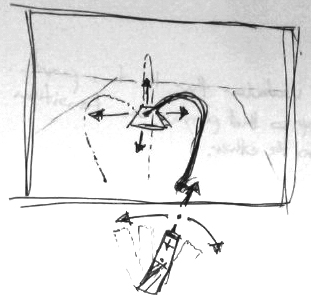
\includegraphics[width=0.4\columnwidth]{img/move}}
\subfloat[finer motion]{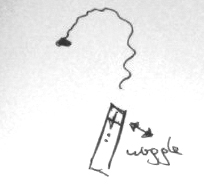
\includegraphics[width=0.4\columnwidth]{img/waggle}}
\caption{Bigger motions are used to apply a pulling force to objects in the scene while finer motions can be used for finer effects like vibrato, etc.}
\label{fig:motion}
\end{figure}


\section{Interaction}
The user interacts with the scene through this \emph{arc of light}. The body is extended into the scene. Interaction occurs on three layers:

\begin{description}
\item[bigger motions] The primary interaction is to apply a pulling force to objects. Movable objects can be dragged around the scene. This is the domain of the arm and the whole body.

\item[finer motions] The second interaction layer comes from finer motions like a slight wiggle of the controller or a subtle rotation. This should enable fine artistic expression. It is the domain of the hand and the fingers. Like the vibrato of a violin player. 

\item[buttons] The final layer are simple button presses, that can be used as well.
\end{description}

\section{Literature Review}
A brief literature review has been performed, but no similar projects could be found. The brief literature review so far covered  \emph{CHI} '07-11, \emph{TEI} '07-11, \emph{SMC} '08-'11, \emph{Computer Music Journal} '07--, \emph{NIME} '10 \& '11.

Further literature review especially in the field of \emph{Tangible User Interfaces} and more general \emph{Virtual and Augmented Reality} is planned.

Appended is the result of the initial search, an uncommented list of potentially relevant literature.

\section{Research Questions}
\begin{enumerate}
\item How can the \emph{arc of light}/fishing rod metaphor be used for intuitive interaction. How does lag impact the system.
\item What meaningful mappings can be derived from the interaction with and the visualisation of the virtual scene.
\end{enumerate}

\section{Learning Goals}
\begin{enumerate}
\item Create a system that allows the user to interact with an virtual world through the \emph{wiimote}. This syststem should be intuitive even for untrained users, and have a very low barrier of entry.
\item Explore the technical capabilities of the \emph{wiimote} and \emph{nunchuck} controller and put it to good use.
\item Create a meaningful mapping form the virtual world to the sound generation system.
\item Create a sound generation system that allows nuanced an rich musical expression.
\item Develop an architecture that streamlines the three stages \emph{input - processing - output}.
\end{enumerate}

\section{Technical Details}
Even though the project is in a very early stage, a few technical characteristics have emerged. However is is very likely that they will change as the project evolves.

The application will be written in \emph{C++} and uses \emph{OpenGL 2.1} to render the virtual scene. \emph{Pure data\footnote{http://puredata.info}} will be used for sound generation, and either \emph{MIDI} or \emph{OSC} will provide the communication link between the two modules.

Primary development platform is \emph{Mac OS X 10.6 Snow Leopard}, on a 64bit Intel processor and an \emph{Intel HD 3000} GPU. Source code is aimed to be platform independent, but the application will not be ported to other platforms during this project. 

\nocite{*}

\bibliographystyle{apalike}
\bibliography{related-work}

\end{document}